%\documentclass{article}
%\usepackage{graphicx,subfigure}
%\begin{document}

\begin{figure}[!h]
  \centering
  \captionsetup{width=0.7\textwidth}
%  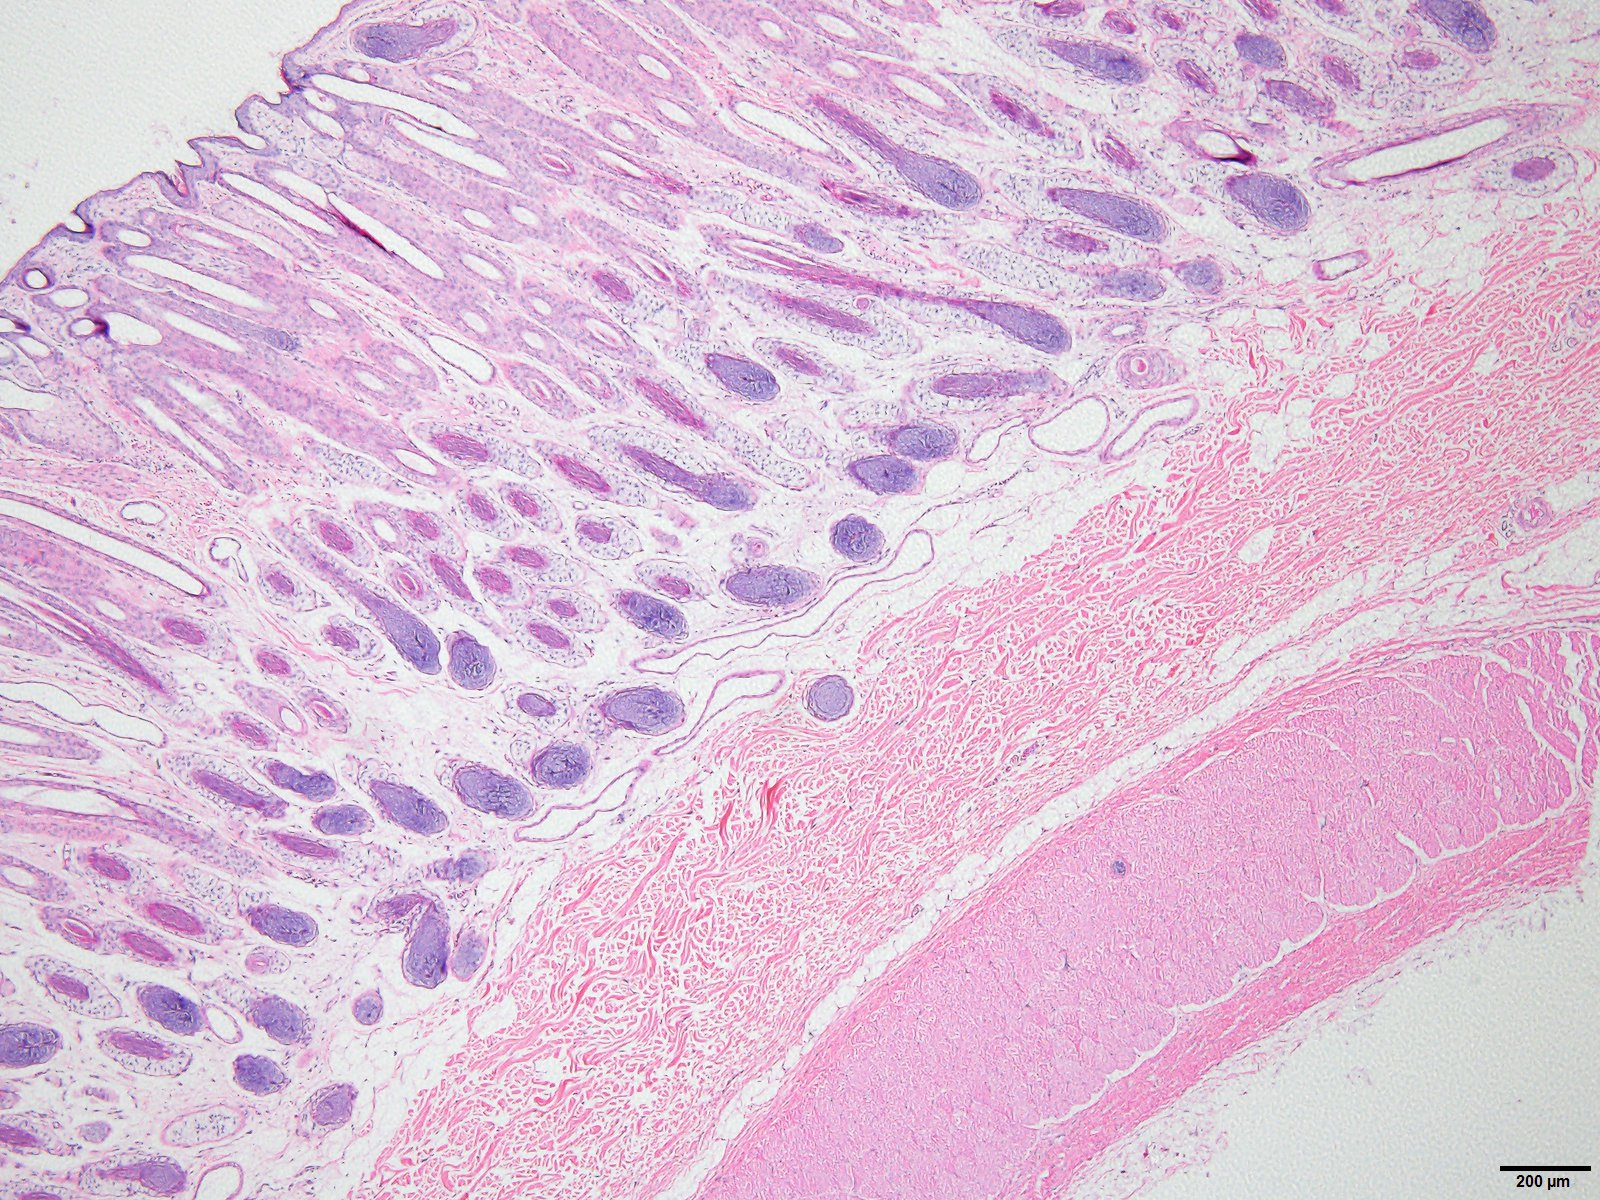
\includegraphics[width=1.0\textwidth]{3456_4layers_4x.jpg}
  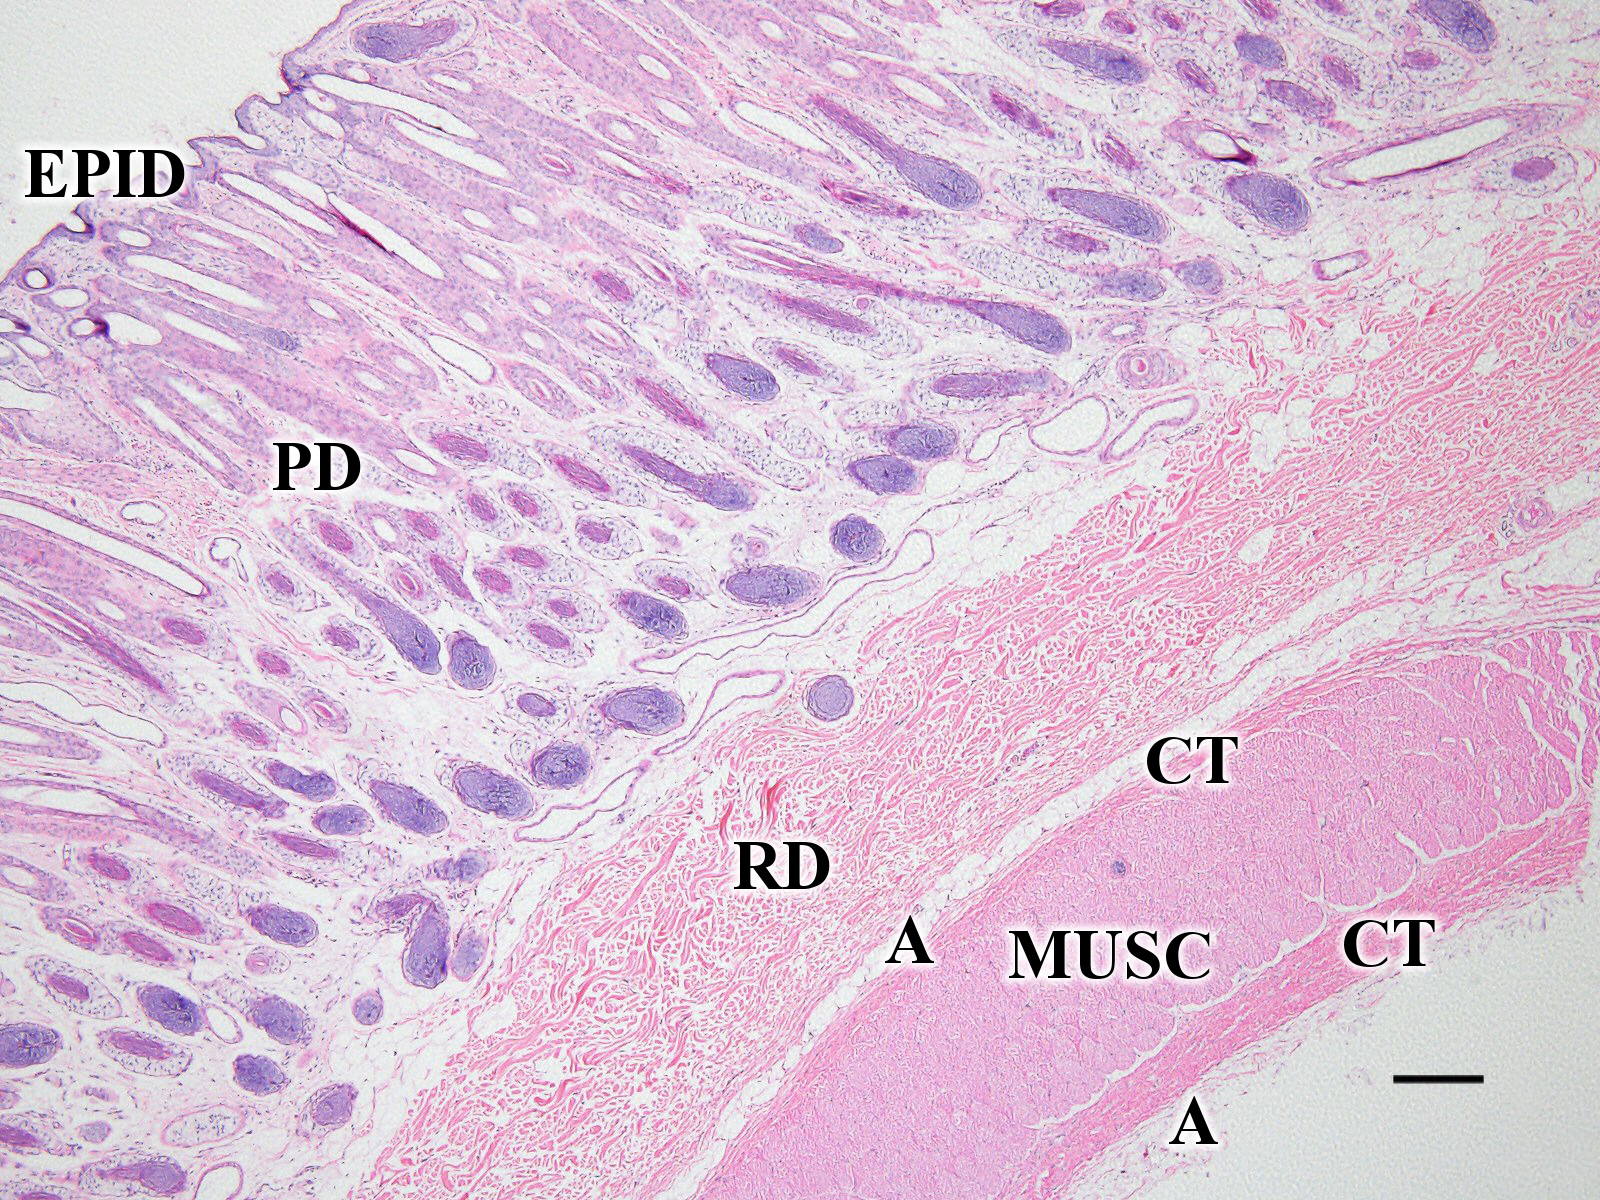
\includegraphics[width=0.7\textwidth]{fig3.jpg}
% 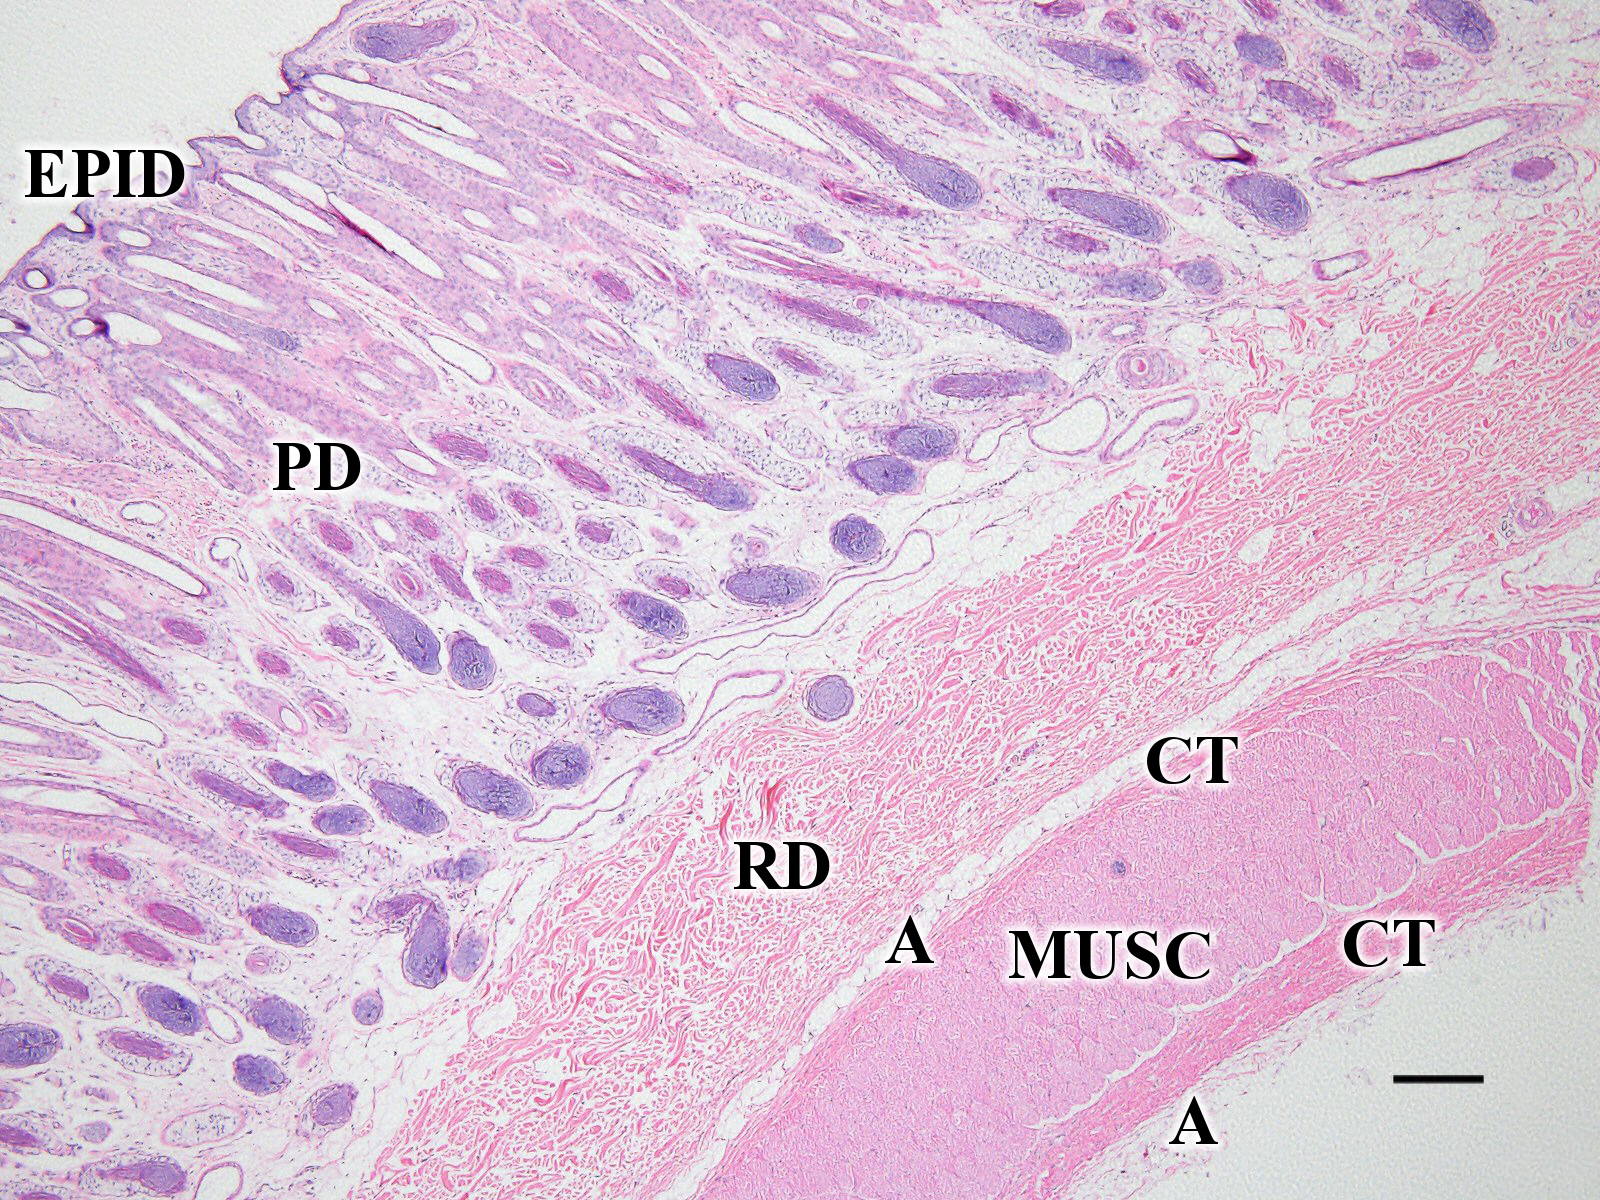
\includegraphics[scale=0.10]{fig3.jpg}
  \caption{Vertical section from a wrinkled sheep (3456) from Trial 2 Flock 1 stained with H-E. This section is from an untrimmed biopsy specimen and shows all 5 layers  identified by Mitchell: {\bf EPID} epidermis, {\bf PD} papillary dermis, {\bf RD} reticular dermis, {\bf MUSC} muscle, and {\bf A} adipose tissue). In addition there are two layers of {\bf CT} connective tissue, either side of the muscle layer, and a thin layer of {\bf A} adipose tissue between the reticular dermis and the muscle. Scale bar is $200\mu m$.}
  \label{fig:trial2he}
\end{figure}

%\end{document}

